% Created by tikzDevice version 0.12.6 on 2024-12-17 18:05:46
% !TEX encoding = UTF-8 Unicode
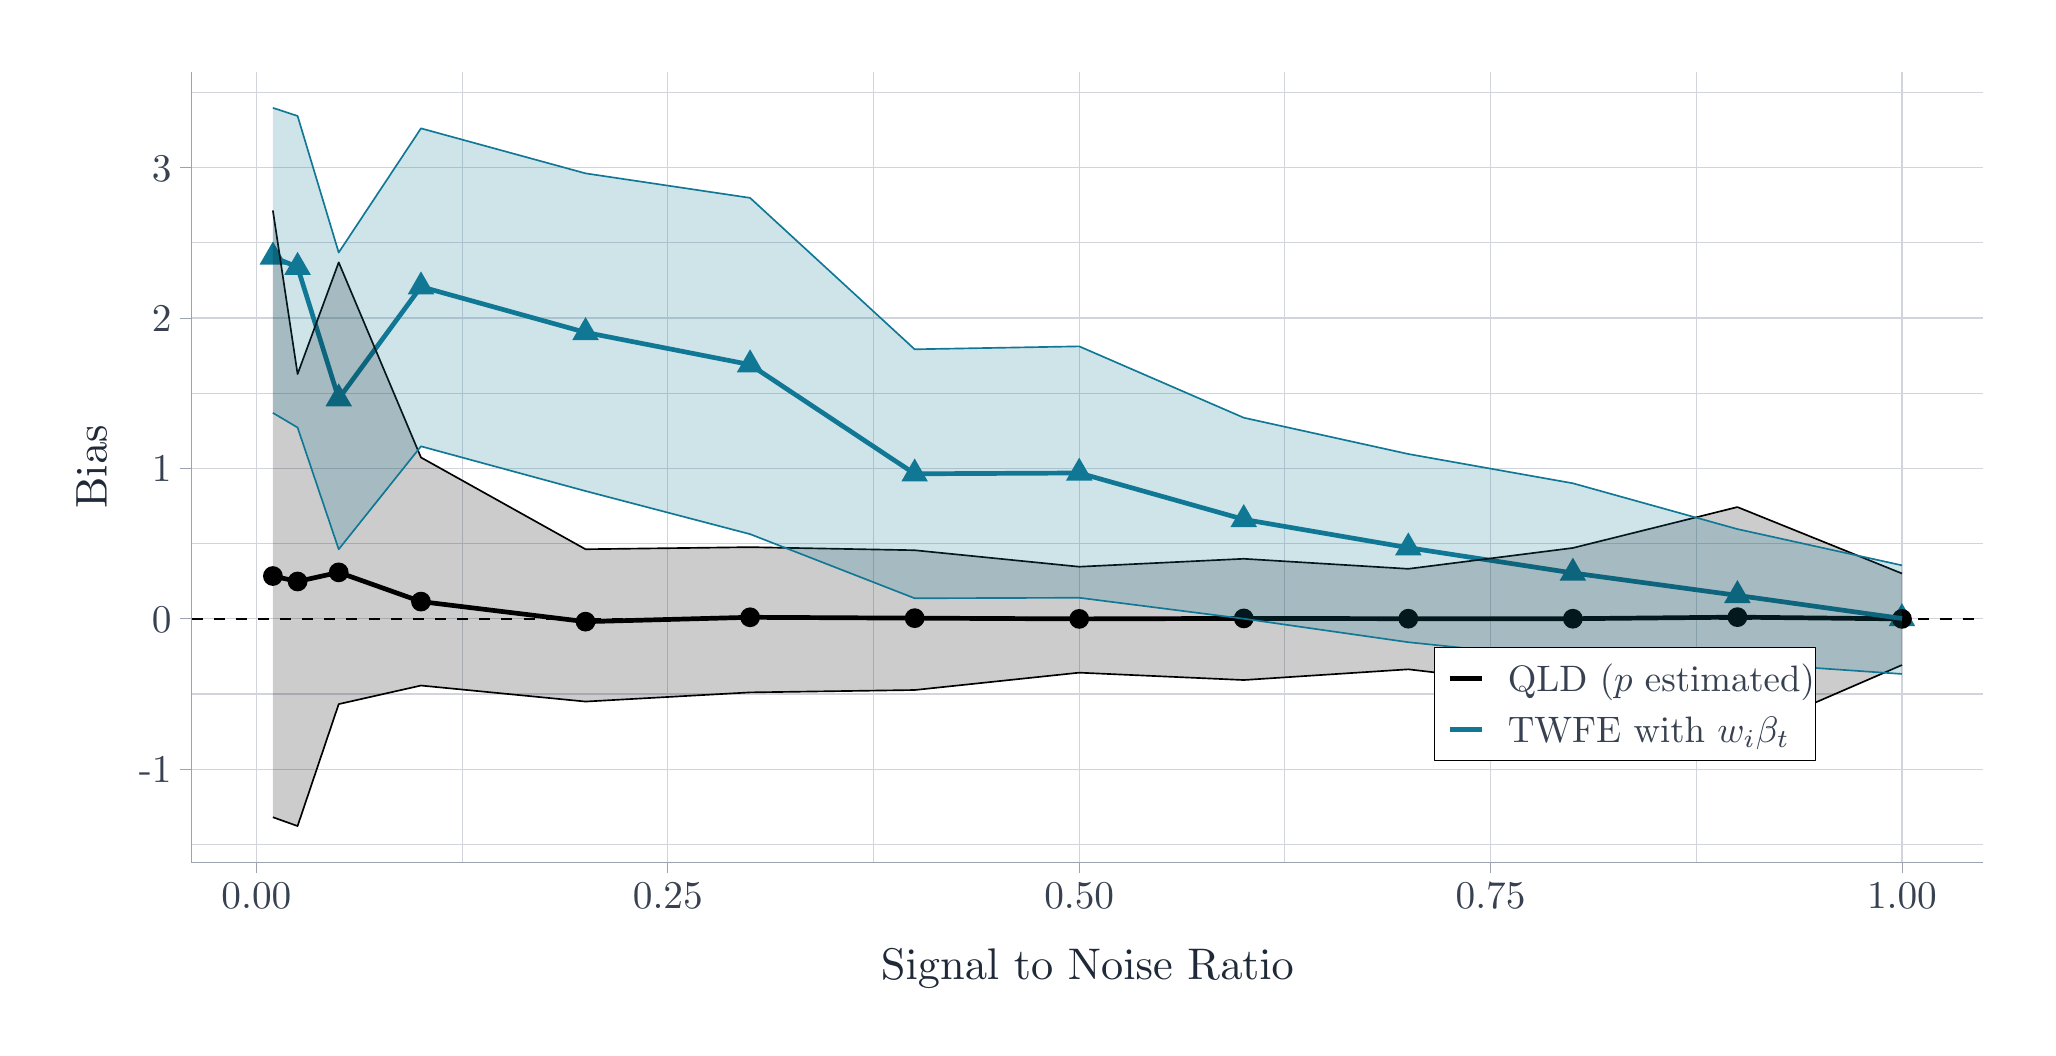
\begin{tikzpicture}[x=1pt,y=1pt]
\definecolor{fillColor}{RGB}{255,255,255}
\path[use as bounding box,fill=fillColor] (0,0) rectangle (722.70,361.35);
\begin{scope}
\path[clip] (  0.00,  0.00) rectangle (722.70,361.35);
\definecolor{drawColor}{RGB}{255,255,255}

\path[draw=drawColor,line width= 0.8pt,line join=round,line cap=round,fill=fillColor] (  0.00,  0.00) rectangle (722.70,361.35);
\end{scope}
\begin{scope}
\path[clip] ( 59.18, 59.89) rectangle (706.70,345.35);
\definecolor{drawColor}{RGB}{255,255,255}
\definecolor{fillColor}{RGB}{255,255,255}

\path[draw=drawColor,line width= 0.8pt,line join=round,line cap=round,fill=fillColor] ( 59.18, 59.89) rectangle (706.70,345.35);
\definecolor{drawColor}{RGB}{209,213,219}

\path[draw=drawColor,line width= 0.4pt,line join=round] ( 59.18, 66.20) --
	(706.70, 66.20);

\path[draw=drawColor,line width= 0.4pt,line join=round] ( 59.18,120.56) --
	(706.70,120.56);

\path[draw=drawColor,line width= 0.4pt,line join=round] ( 59.18,174.91) --
	(706.70,174.91);

\path[draw=drawColor,line width= 0.4pt,line join=round] ( 59.18,229.27) --
	(706.70,229.27);

\path[draw=drawColor,line width= 0.4pt,line join=round] ( 59.18,283.62) --
	(706.70,283.62);

\path[draw=drawColor,line width= 0.4pt,line join=round] ( 59.18,337.97) --
	(706.70,337.97);

\path[draw=drawColor,line width= 0.4pt,line join=round] (156.99, 59.89) --
	(156.99,345.35);

\path[draw=drawColor,line width= 0.4pt,line join=round] (305.64, 59.89) --
	(305.64,345.35);

\path[draw=drawColor,line width= 0.4pt,line join=round] (454.29, 59.89) --
	(454.29,345.35);

\path[draw=drawColor,line width= 0.4pt,line join=round] (602.94, 59.89) --
	(602.94,345.35);

\path[draw=drawColor,line width= 0.4pt,line join=round] ( 59.18, 93.38) --
	(706.70, 93.38);

\path[draw=drawColor,line width= 0.4pt,line join=round] ( 59.18,147.73) --
	(706.70,147.73);

\path[draw=drawColor,line width= 0.4pt,line join=round] ( 59.18,202.09) --
	(706.70,202.09);

\path[draw=drawColor,line width= 0.4pt,line join=round] ( 59.18,256.44) --
	(706.70,256.44);

\path[draw=drawColor,line width= 0.4pt,line join=round] ( 59.18,310.80) --
	(706.70,310.80);

\path[draw=drawColor,line width= 0.4pt,line join=round] ( 82.66, 59.89) --
	( 82.66,345.35);

\path[draw=drawColor,line width= 0.4pt,line join=round] (231.31, 59.89) --
	(231.31,345.35);

\path[draw=drawColor,line width= 0.4pt,line join=round] (379.97, 59.89) --
	(379.97,345.35);

\path[draw=drawColor,line width= 0.4pt,line join=round] (528.62, 59.89) --
	(528.62,345.35);

\path[draw=drawColor,line width= 0.4pt,line join=round] (677.27, 59.89) --
	(677.27,345.35);
\definecolor{drawColor}{RGB}{0,0,0}

\path[draw=drawColor,line width= 0.6pt,dash pattern=on 4pt off 4pt ,line join=round] ( 59.18,147.73) -- (706.70,147.73);
\definecolor{fillColor}{RGB}{16,120,149}

\path[fill=fillColor] ( 88.61,284.07) --
	( 93.42,275.75) --
	( 83.80,275.75) --
	cycle;
\definecolor{fillColor}{RGB}{0,0,0}

\path[fill=fillColor] ( 88.61,163.20) circle (  3.57);
\definecolor{fillColor}{RGB}{16,120,149}

\path[fill=fillColor] ( 97.53,280.36) --
	(102.33,272.03) --
	( 92.72,272.03) --
	cycle;
\definecolor{fillColor}{RGB}{0,0,0}

\path[fill=fillColor] ( 97.53,161.23) circle (  3.57);
\definecolor{fillColor}{RGB}{16,120,149}

\path[fill=fillColor] (112.39,232.82) --
	(117.20,224.50) --
	(107.59,224.50) --
	cycle;
\definecolor{fillColor}{RGB}{0,0,0}

\path[fill=fillColor] (112.39,164.52) circle (  3.57);
\definecolor{fillColor}{RGB}{16,120,149}

\path[fill=fillColor] (142.12,273.29) --
	(146.93,264.96) --
	(137.32,264.96) --
	cycle;
\definecolor{fillColor}{RGB}{0,0,0}

\path[fill=fillColor] (142.12,153.96) circle (  3.57);
\definecolor{fillColor}{RGB}{16,120,149}

\path[fill=fillColor] (201.58,256.78) --
	(206.39,248.46) --
	(196.78,248.46) --
	cycle;
\definecolor{fillColor}{RGB}{0,0,0}

\path[fill=fillColor] (201.58,146.71) circle (  3.57);
\definecolor{fillColor}{RGB}{16,120,149}

\path[fill=fillColor] (261.04,245.14) --
	(265.85,236.81) --
	(256.24,236.81) --
	cycle;
\definecolor{fillColor}{RGB}{0,0,0}

\path[fill=fillColor] (261.04,148.29) circle (  3.57);
\definecolor{fillColor}{RGB}{16,120,149}

\path[fill=fillColor] (320.51,205.69) --
	(325.31,197.37) --
	(315.70,197.37) --
	cycle;
\definecolor{fillColor}{RGB}{0,0,0}

\path[fill=fillColor] (320.51,147.98) circle (  3.57);
\definecolor{fillColor}{RGB}{16,120,149}

\path[fill=fillColor] (379.97,205.98) --
	(384.77,197.66) --
	(375.16,197.66) --
	cycle;
\definecolor{fillColor}{RGB}{0,0,0}

\path[fill=fillColor] (379.97,147.71) circle (  3.57);
\definecolor{fillColor}{RGB}{16,120,149}

\path[fill=fillColor] (439.43,189.21) --
	(444.23,180.89) --
	(434.62,180.89) --
	cycle;
\definecolor{fillColor}{RGB}{0,0,0}

\path[fill=fillColor] (439.43,147.88) circle (  3.57);
\definecolor{fillColor}{RGB}{16,120,149}

\path[fill=fillColor] (498.89,178.98) --
	(503.69,170.66) --
	(494.08,170.66) --
	cycle;
\definecolor{fillColor}{RGB}{0,0,0}

\path[fill=fillColor] (498.89,147.78) circle (  3.57);
\definecolor{fillColor}{RGB}{16,120,149}

\path[fill=fillColor] (558.35,169.85) --
	(563.15,161.52) --
	(553.54,161.52) --
	cycle;
\definecolor{fillColor}{RGB}{0,0,0}

\path[fill=fillColor] (558.35,147.78) circle (  3.57);
\definecolor{fillColor}{RGB}{16,120,149}

\path[fill=fillColor] (617.81,161.75) --
	(622.61,153.43) --
	(613.00,153.43) --
	cycle;
\definecolor{fillColor}{RGB}{0,0,0}

\path[fill=fillColor] (617.81,148.34) circle (  3.57);
\definecolor{fillColor}{RGB}{16,120,149}

\path[fill=fillColor] (677.27,153.40) --
	(682.07,145.07) --
	(672.46,145.07) --
	cycle;
\definecolor{fillColor}{RGB}{0,0,0}

\path[fill=fillColor] (677.27,147.71) circle (  3.57);

\path[draw=drawColor,line width= 1.7pt,line join=round] ( 88.61,163.20) --
	( 97.53,161.23) --
	(112.39,164.52) --
	(142.12,153.96) --
	(201.58,146.71) --
	(261.04,148.29) --
	(320.51,147.98) --
	(379.97,147.71) --
	(439.43,147.88) --
	(498.89,147.78) --
	(558.35,147.78) --
	(617.81,148.34) --
	(677.27,147.71);
\definecolor{drawColor}{RGB}{16,120,149}

\path[draw=drawColor,line width= 1.7pt,line join=round] ( 88.61,278.52) --
	( 97.53,274.81) --
	(112.39,227.27) --
	(142.12,267.74) --
	(201.58,251.23) --
	(261.04,239.59) --
	(320.51,200.14) --
	(379.97,200.43) --
	(439.43,183.66) --
	(498.89,173.43) --
	(558.35,164.30) --
	(617.81,156.20) --
	(677.27,147.85);
\definecolor{fillColor}{RGB}{0,0,0}

\path[fill=fillColor,fill opacity=0.20] ( 88.61,295.29) --
	( 97.53,236.18) --
	(112.39,276.54) --
	(142.12,206.04) --
	(201.58,172.88) --
	(261.04,173.63) --
	(320.51,172.52) --
	(379.97,166.56) --
	(439.43,169.43) --
	(498.89,165.80) --
	(558.35,173.34) --
	(617.81,188.12) --
	(677.27,164.12) --
	(677.27,131.04) --
	(617.81,105.28) --
	(558.35,122.55) --
	(498.89,129.49) --
	(439.43,125.62) --
	(379.97,128.28) --
	(320.51,122.01) --
	(261.04,121.15) --
	(201.58,117.84) --
	(142.12,123.63) --
	(112.39,116.92) --
	( 97.53, 72.86) --
	( 88.61, 76.04) --
	cycle;
\definecolor{drawColor}{RGB}{0,0,0}

\path[draw=drawColor,line width= 0.6pt,line join=round] ( 88.61,295.29) --
	( 97.53,236.18) --
	(112.39,276.54) --
	(142.12,206.04) --
	(201.58,172.88) --
	(261.04,173.63) --
	(320.51,172.52) --
	(379.97,166.56) --
	(439.43,169.43) --
	(498.89,165.80) --
	(558.35,173.34) --
	(617.81,188.12) --
	(677.27,164.12);

\path[draw=drawColor,line width= 0.6pt,line join=round] (677.27,131.04) --
	(617.81,105.28) --
	(558.35,122.55) --
	(498.89,129.49) --
	(439.43,125.62) --
	(379.97,128.28) --
	(320.51,122.01) --
	(261.04,121.15) --
	(201.58,117.84) --
	(142.12,123.63) --
	(112.39,116.92) --
	( 97.53, 72.86) --
	( 88.61, 76.04);
\definecolor{fillColor}{RGB}{16,120,149}

\path[fill=fillColor,fill opacity=0.20] ( 88.61,332.37) --
	( 97.53,329.44) --
	(112.39,280.09) --
	(142.12,324.96) --
	(201.58,308.70) --
	(261.04,299.84) --
	(320.51,245.13) --
	(379.97,246.19) --
	(439.43,220.40) --
	(498.89,207.29) --
	(558.35,196.71) --
	(617.81,180.16) --
	(677.27,167.06) --
	(677.27,127.81) --
	(617.81,131.92) --
	(558.35,133.15) --
	(498.89,139.28) --
	(439.43,147.77) --
	(379.97,155.35) --
	(320.51,155.16) --
	(261.04,178.34) --
	(201.58,193.91) --
	(142.12,210.07) --
	(112.39,172.85) --
	( 97.53,216.86) --
	( 88.61,222.15) --
	cycle;
\definecolor{drawColor}{RGB}{16,120,149}

\path[draw=drawColor,line width= 0.6pt,line join=round] ( 88.61,332.37) --
	( 97.53,329.44) --
	(112.39,280.09) --
	(142.12,324.96) --
	(201.58,308.70) --
	(261.04,299.84) --
	(320.51,245.13) --
	(379.97,246.19) --
	(439.43,220.40) --
	(498.89,207.29) --
	(558.35,196.71) --
	(617.81,180.16) --
	(677.27,167.06);

\path[draw=drawColor,line width= 0.6pt,line join=round] (677.27,127.81) --
	(617.81,131.92) --
	(558.35,133.15) --
	(498.89,139.28) --
	(439.43,147.77) --
	(379.97,155.35) --
	(320.51,155.16) --
	(261.04,178.34) --
	(201.58,193.91) --
	(142.12,210.07) --
	(112.39,172.85) --
	( 97.53,216.86) --
	( 88.61,222.15);
\end{scope}
\begin{scope}
\path[clip] (  0.00,  0.00) rectangle (722.70,361.35);
\definecolor{drawColor}{RGB}{156,163,175}

\path[draw=drawColor,line width= 0.3pt,line join=round] ( 59.18, 59.89) --
	( 59.18,345.35);
\end{scope}
\begin{scope}
\path[clip] (  0.00,  0.00) rectangle (722.70,361.35);
\definecolor{drawColor}{RGB}{55,65,81}

\node[text=drawColor,anchor=base east,inner sep=0pt, outer sep=0pt, scale=  1.42] at ( 51.98, 88.48) {-1};

\node[text=drawColor,anchor=base east,inner sep=0pt, outer sep=0pt, scale=  1.42] at ( 51.98,142.84) {0};

\node[text=drawColor,anchor=base east,inner sep=0pt, outer sep=0pt, scale=  1.42] at ( 51.98,197.19) {1};

\node[text=drawColor,anchor=base east,inner sep=0pt, outer sep=0pt, scale=  1.42] at ( 51.98,251.55) {2};

\node[text=drawColor,anchor=base east,inner sep=0pt, outer sep=0pt, scale=  1.42] at ( 51.98,305.90) {3};
\end{scope}
\begin{scope}
\path[clip] (  0.00,  0.00) rectangle (722.70,361.35);
\definecolor{drawColor}{RGB}{156,163,175}

\path[draw=drawColor,line width= 0.3pt,line join=round] ( 55.18, 93.38) --
	( 59.18, 93.38);

\path[draw=drawColor,line width= 0.3pt,line join=round] ( 55.18,147.73) --
	( 59.18,147.73);

\path[draw=drawColor,line width= 0.3pt,line join=round] ( 55.18,202.09) --
	( 59.18,202.09);

\path[draw=drawColor,line width= 0.3pt,line join=round] ( 55.18,256.44) --
	( 59.18,256.44);

\path[draw=drawColor,line width= 0.3pt,line join=round] ( 55.18,310.80) --
	( 59.18,310.80);
\end{scope}
\begin{scope}
\path[clip] (  0.00,  0.00) rectangle (722.70,361.35);
\definecolor{drawColor}{RGB}{156,163,175}

\path[draw=drawColor,line width= 0.3pt,line join=round] ( 59.18, 59.89) --
	(706.70, 59.89);
\end{scope}
\begin{scope}
\path[clip] (  0.00,  0.00) rectangle (722.70,361.35);
\definecolor{drawColor}{RGB}{156,163,175}

\path[draw=drawColor,line width= 0.3pt,line join=round] ( 82.66, 55.89) --
	( 82.66, 59.89);

\path[draw=drawColor,line width= 0.3pt,line join=round] (231.31, 55.89) --
	(231.31, 59.89);

\path[draw=drawColor,line width= 0.3pt,line join=round] (379.97, 55.89) --
	(379.97, 59.89);

\path[draw=drawColor,line width= 0.3pt,line join=round] (528.62, 55.89) --
	(528.62, 59.89);

\path[draw=drawColor,line width= 0.3pt,line join=round] (677.27, 55.89) --
	(677.27, 59.89);
\end{scope}
\begin{scope}
\path[clip] (  0.00,  0.00) rectangle (722.70,361.35);
\definecolor{drawColor}{RGB}{55,65,81}

\node[text=drawColor,anchor=base,inner sep=0pt, outer sep=0pt, scale=  1.42] at ( 82.66, 42.89) {0.00};

\node[text=drawColor,anchor=base,inner sep=0pt, outer sep=0pt, scale=  1.42] at (231.31, 42.89) {0.25};

\node[text=drawColor,anchor=base,inner sep=0pt, outer sep=0pt, scale=  1.42] at (379.97, 42.89) {0.50};

\node[text=drawColor,anchor=base,inner sep=0pt, outer sep=0pt, scale=  1.42] at (528.62, 42.89) {0.75};

\node[text=drawColor,anchor=base,inner sep=0pt, outer sep=0pt, scale=  1.42] at (677.27, 42.89) {1.00};
\end{scope}
\begin{scope}
\path[clip] (  0.00,  0.00) rectangle (722.70,361.35);
\definecolor{drawColor}{RGB}{31,41,55}

\node[text=drawColor,anchor=base,inner sep=0pt, outer sep=0pt, scale=  1.60] at (382.94, 17.56) {Signal to Noise Ratio};
\end{scope}
\begin{scope}
\path[clip] (  0.00,  0.00) rectangle (722.70,361.35);
\definecolor{drawColor}{RGB}{31,41,55}

\node[text=drawColor,rotate= 90.00,anchor=base,inner sep=0pt, outer sep=0pt, scale=  1.60] at ( 28.57,202.62) {Bias};
\end{scope}
\begin{scope}
\path[clip] (  0.00,  0.00) rectangle (722.70,361.35);
\definecolor{drawColor}{RGB}{0,0,0}
\definecolor{fillColor}{RGB}{255,255,255}

\path[draw=drawColor,line width= 0.6pt,line join=round,line cap=round,fill=fillColor] (508.38, 96.53) rectangle (646.01,137.43);
\end{scope}
\begin{scope}
\path[clip] (  0.00,  0.00) rectangle (722.70,361.35);
\definecolor{drawColor}{RGB}{255,255,255}
\definecolor{fillColor}{RGB}{255,255,255}

\path[draw=drawColor,line width= 0.8pt,line join=round,line cap=round,fill=fillColor] (512.38,118.98) rectangle (526.84,133.43);
\end{scope}
\begin{scope}
\path[clip] (  0.00,  0.00) rectangle (722.70,361.35);
\definecolor{fillColor}{RGB}{0,0,0}

\path[fill=fillColor] (519.61,126.21) circle (  0.36);
\end{scope}
\begin{scope}
\path[clip] (  0.00,  0.00) rectangle (722.70,361.35);
\definecolor{drawColor}{RGB}{0,0,0}

\path[draw=drawColor,line width= 1.7pt,line join=round] (513.83,126.21) -- (525.39,126.21);
\end{scope}
\begin{scope}
\path[clip] (  0.00,  0.00) rectangle (722.70,361.35);
\definecolor{drawColor}{RGB}{255,255,255}
\definecolor{fillColor}{RGB}{255,255,255}

\path[draw=drawColor,line width= 0.8pt,line join=round,line cap=round,fill=fillColor] (512.38,100.53) rectangle (526.84,114.98);
\end{scope}
\begin{scope}
\path[clip] (  0.00,  0.00) rectangle (722.70,361.35);
\definecolor{fillColor}{RGB}{16,120,149}

\path[fill=fillColor] (519.61,108.31) --
	(520.09,107.48) --
	(519.13,107.48) --
	cycle;
\end{scope}
\begin{scope}
\path[clip] (  0.00,  0.00) rectangle (722.70,361.35);
\definecolor{drawColor}{RGB}{16,120,149}

\path[draw=drawColor,line width= 1.7pt,line join=round] (513.83,107.75) -- (525.39,107.75);
\end{scope}
\begin{scope}
\path[clip] (  0.00,  0.00) rectangle (722.70,361.35);
\definecolor{drawColor}{RGB}{55,65,81}

\node[text=drawColor,anchor=base west,inner sep=0pt, outer sep=0pt, scale=  1.33] at (534.84,121.62) {QLD ($p$ estimated)};
\end{scope}
\begin{scope}
\path[clip] (  0.00,  0.00) rectangle (722.70,361.35);
\definecolor{drawColor}{RGB}{55,65,81}

\node[text=drawColor,anchor=base west,inner sep=0pt, outer sep=0pt, scale=  1.33] at (534.84,103.16) {TWFE with $\bm{w}_i \beta_t$};
\end{scope}
\end{tikzpicture}
